\section{Divide and Conquer}
\subsection*{Integer Multiplication}

Imagine multiplying an n-bit number by another n-bit
number, where n is a perfect power of 2.
(This will make the analysis easier.)
We can split up each of these numbers into two halves. 

$I\times J=[(I_h\times 2^{\frac{n}{2}}+I_l)]\times[(J_h\times 2^{\frac{n}{2}}+J_l)]=%
I_h\times J_h\times 2^n+(I_l\times J_h+I_h\times J_l)\times 2^{\frac{n}{2}}+I_l\times J_l$

This way, we have broken down the problem of 2 n-bit nums into 4 mults of
n/2-bit nums plus 3 addtions.
Thus the run-time $T(n)=4T(n/2)+\theta(n)$

This has the solution of $T(n)=\theta(n^2)$ by the Master Theorem.

To optimize this:

$P_1=(I_h+I_l)\times(J_h+J_l)=I_h\times J_h+I_x\times J_l+I_l\times J_h+I_l\times J_l$


$P_2=I_h\times J_h$

$P_3=I_l\times J_l$

$P_1-P_2-P_3=I_h\times J_1+I_l\times J_h$

$I\times J=P_2\times 2^n+[P_1-P_2-P_3]\times 2^{\frac{n}{2}}+P_3$

\subsection*{Tromino "Tiling"}
A tromino is a figure composed of three 1x1 squares in the shape of an L.
Given a $2^n\times 2^n$ checkerboard with 1 missing square, we can recursively tile that 
square with trominoes.

\begin{enumerate}
    \item Split the board into four equal sized squares.
    \item The missing square is in one of these four squares.
        Recursively tile this square since it is a proper recursive case.
    \item Although the three other squares aren't missing squares, we can "create"
        these recursive cases by tiling one tronimo in the center of the board,
        where appropriate:
\end{enumerate}

\resizebox{\linewidth}{!}{%
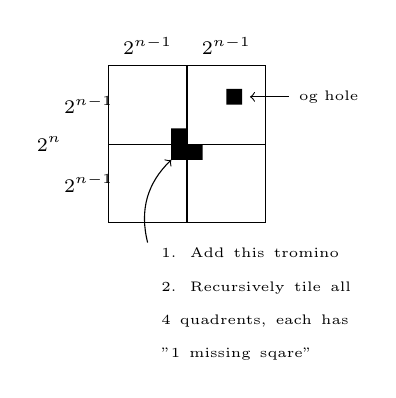
\begin{tikzpicture}

    \foreach \x/ \y in {0.5/2.25, 1.5/2.25, -0.25/0.5, -0.25/1.5} {
        \node () at (\x,\y) {\scriptsize $\cramped{2^{n-1}}$};
    };

    \node () at (-0.75,1) {\scriptsize $2^n$};

    \path[draw] (0,0) rectangle ++(2,2)
        (1,0) -- +(0,2)
        (0,1) -- +(2,0);

    \path[<-,fill]
        % o.g. hole
        (1.5,1.5) rectangle ++(0.2,0.2)
        ++(0.1,-0.1) edge +(.5,0) ++(0.5,0) node[right] () {\tiny og hole}
        (1,1) rectangle ++(-0.2,0.2)
        (1,1) rectangle ++(0.2,-0.2)
        (1,1) rectangle ++(-0.2,-0.2)
        edge[bend right=30] (0.5,-0.25) ++(-0.25,-1) node[below right,text width=7em] () {\tiny 1. Add this tromino\\ 2. Recursively tile all 4 quadrents, each has "1 missing sqare"};
\end{tikzpicture}
}

\subsection*{Skyline Problem}
\lipsum[1][1-2]
\subsection*{Closest Pair of Points}
The Closest Pair of Points Algorithm is an O(nlogn) solution to the problem of finding the closest pair of points
when given a set of points with (x,y) coordinates. It has a base case of 2 points and a second base case of 3 points.
Base case size 3 uses a brute force algorithm to return the closest pair. Base case size 2 returns that the distance between the two points.
\begin{enumerate}
    \item Sort the points based on their x coordinates (Use merge or quick)
    \item Recursively split the sorted array in halves (like a merge sort does) until the base case of 3 or 2 is met.
    \item To merge the halves, find the minimum distance out of the two halves, and label it delta. 
    \item Create an Array of all of the points within 'delta' distance of the halfway line.
    \item Sort this array based on the y coordinates (use merge or quick).
    \item Brute force search for the smallest distance within this array (Max size of array is 8) 
    \item This smallest distance is the true smallest distance for this section. Repeat the process.
\end{enumerate}
\subsection*{Strassen's Algorithm}
\lipsum[1][1-2]
